\chapter{SYSTEM DESIGN}

\section{System Requirements}

\subsection{Functional Requirements}

The student forum application implements the following core functional capabilities:

\subsubsection{User Management}
\begin{itemize}
    \item \textbf{FR-1}: User registration with email verification - The system shall allow new users to create accounts by providing email, username, and password credentials, followed by mandatory email verification before account activation.
    \item \textbf{FR-2}: Secure user authentication - The system shall authenticate users through secure login mechanisms using Supabase authentication services with session-based state management.
    \item \textbf{FR-3}: Profile management - Users shall be able to view and update their profile information including personal details and forum preferences.
    \item \textbf{FR-4}: Session management - The system shall maintain user sessions securely with automatic timeout and proper session invalidation upon logout.
\end{itemize}

\subsubsection{Content Management}
\begin{itemize}
    \item \textbf{FR-5}: Multi-type post creation - Authenticated users shall be able to create, edit, and delete three types of forum posts: basic text posts, interactive polls with multiple options, and event posts with date/time and location information.
    \item \textbf{FR-6}: Comment system - Users shall be able to add, edit, and delete comments on forum posts with proper threading and moderation capabilities.
    \item \textbf{FR-7}: Content search - The system shall provide advanced search functionality to locate posts and comments based on keywords, filters, and content type with real-time suggestions.
    \item \textbf{FR-8}: Channel management system - The system shall organize posts into channels with approval workflows, channel categories (general, academic, social, announcements), and speciality-specific channels for targeted discussions.
    \item \textbf{FR-15}: Post interaction system - Users shall be able to upvote and downvote posts and comments to promote quality content and community-driven content curation.
    \item \textbf{FR-16}: Student verification system - The system shall verify student status through university email verification and student card validation (pending approval process) to distinguish verified students from general users.
\end{itemize}

\subsubsection{Academic Services}
\begin{itemize}
    \item \textbf{FR-17}: Course review system - Verified students shall be able to review courses per speciality with ratings and written feedback to help fellow students make informed academic decisions.
    \item \textbf{FR-18}: Professor search and evaluation - The system shall provide a searchable database of professors with aggregated ratings, reviews, and course associations for academic planning.
\end{itemize}

\subsubsection{Future Features (Planned)}
\begin{itemize}
    \item \textbf{FR-19}: Location-based channels - The system shall support local channels that display posts based on geographic proximity to enhance campus-specific discussions (future implementation).
    \item \textbf{FR-20}: Personal schedule integration - Users shall be able to import and manage personal calendars with course schedules and event integration (future implementation).
\end{itemize}

\subsubsection{Security and Access Control}
\begin{itemize}
    \item \textbf{FR-9}: Role-based access control - The system shall implement three user roles: verified students (university email verification), unverified users (limited access), and admin users, with appropriate permissions for content management and administrative functions.
    \item \textbf{FR-10}: Input validation and sanitization - All user inputs shall be validated server-side and sanitized to prevent injection attacks and ensure data integrity.
    \item \textbf{FR-11}: Secure API endpoints - All API routes shall require proper authentication and authorization before processing requests.
    \item \textbf{FR-12}: Professor and student rating system with leaderboards - Verified students shall be able to rate professors across multiple categories (teaching quality, communication, helpfulness) and rate fellow students in categories (academic help, collaboration, leadership, social), with anonymous review capabilities and leaderboard displays based on ratings.
    \item \textbf{FR-13}: Content recommendation system - The system shall provide intelligent content recommendations to users based on their academic speciality, interaction history, and channel preferences to enhance content discovery and engagement.
    \item \textbf{FR-14}: Audit logging - The system shall log user activities and security events for monitoring and compliance purposes.
\end{itemize}

\subsection{Non-Functional Requirements}

The application addresses critical security and performance requirements essential for a secure educational platform:

\subsubsection{Security Requirements}
\begin{itemize}
    \item \textbf{NFR-1}: Encryption standards - All data transmission shall be encrypted using TLS 1.3, and sensitive data at rest shall be encrypted using AES-256 encryption algorithms.
    \item \textbf{NFR-2}: Password security - User passwords shall be hashed using bcrypt with a minimum of 12 salt rounds, and password policies shall enforce strong password requirements.
    \item \textbf{NFR-3}: Cross-Site Scripting (XSS) prevention - The application shall implement Content Security Policy (CSP) headers and input sanitization to prevent XSS attacks.
    \item \textbf{NFR-4}: Cross-Site Request Forgery (CSRF) protection - All state-changing operations shall be protected with anti-CSRF tokens and same-site cookie attributes.
    \item \textbf{NFR-5}: SQL injection prevention - Database operations shall use parameterized queries through Drizzle ORM to prevent SQL injection vulnerabilities.
    \item \textbf{NFR-6}: Session security - Sessions shall implement secure cookie attributes (HttpOnly, Secure, SameSite) with automatic timeout after 24 hours of inactivity.
\end{itemize}

\subsubsection{Performance Requirements}
\begin{itemize}
    \item \textbf{NFR-7}: Response time - API endpoints shall respond within 500ms for 95\% of requests under normal load conditions.
    \item \textbf{NFR-8}: Scalability - The system shall support concurrent access by up to 1000 authenticated users without performance degradation.
    \item \textbf{NFR-9}: Database performance - Database queries shall be optimized with proper indexing to maintain sub-100ms response times for common operations.
\end{itemize}

\subsubsection{Reliability and Availability}
\begin{itemize}
    \item \textbf{NFR-10}: System availability - The application shall maintain 99.5\% uptime during operational hours with automated failover capabilities.
    \item \textbf{NFR-11}: Data backup - User data and forum content shall be automatically backed up daily with point-in-time recovery capabilities.
    \item \textbf{NFR-12}: Error handling - The system shall implement comprehensive error handling that prevents sensitive information disclosure while providing meaningful feedback to users.
\end{itemize}

\subsubsection{Compliance and Standards}
\begin{itemize}
    \item \textbf{NFR-13}: Security standards compliance - The application shall adhere to OWASP Top 10 security guidelines and implement security best practices throughout the development lifecycle.
    \item \textbf{NFR-14}: Data privacy - User data handling shall comply with educational privacy standards and implement proper data retention policies.
    \item \textbf{NFR-15}: Accessibility - The user interface shall meet WCAG 2.1 Level AA accessibility standards to ensure inclusive access for all users.
\end{itemize}

\section{System Architecture Overview}

The student forum application follows a modern web architecture pattern utilizing Next.js as the full-stack framework, Supabase for authentication and database services, and Drizzle ORM for type-safe database operations. The system employs a component-based design that separates concerns between the frontend presentation layer, server-side business logic, and data persistence layer.

\begin{figure}[H]
\centering
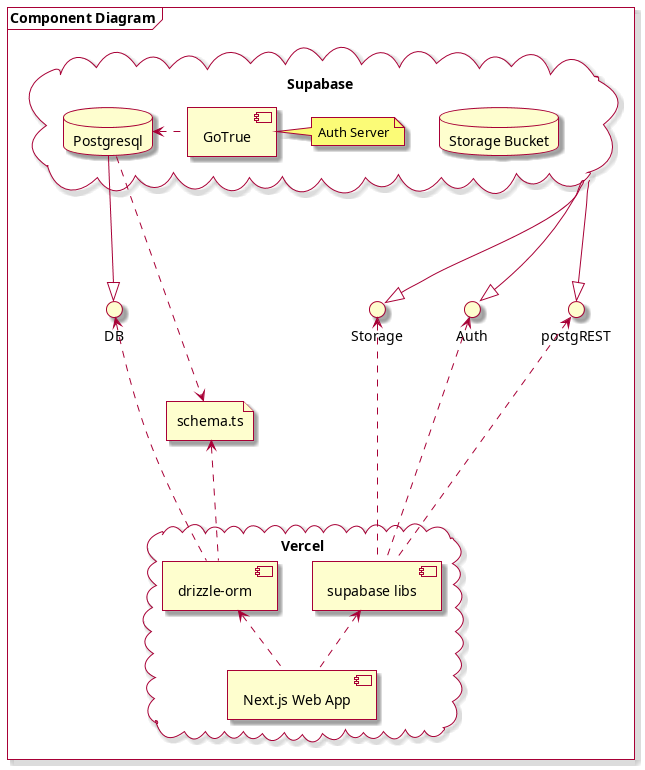
\includegraphics[width=0.8\textwidth]{img/component-diagram.png}
\caption{System Component Architecture}
\label{fig:component-diagram}
\end{figure}

The architecture shown in Figure \ref{fig:component-diagram} demonstrates the interaction between Vercel's hosting environment and Supabase's backend services. The Next.js application utilizes both Drizzle ORM for direct database operations and Supabase libraries for authentication and file storage, creating a hybrid approach that leverages the strengths of each technology.

\section{Application Feature Design}

The Next.js application follows a feature-based architecture where functionality is organized into distinct, modular components that interact through well-defined interfaces. This approach promotes code reusability, maintainability, and separation of concerns.

\begin{figure}[H]
\centering
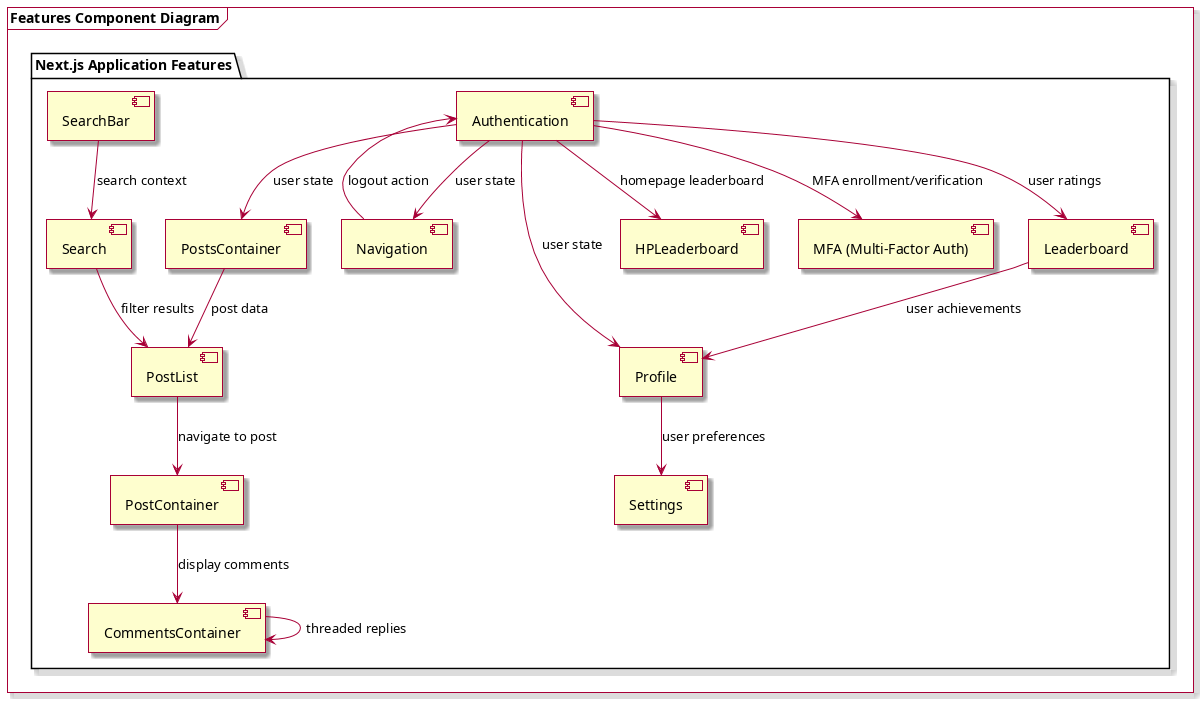
\includegraphics[width=0.8\textwidth]{img/features-component.png}
\caption{Application Features Component Diagram}
\label{fig:features-component}
\end{figure}

The feature architecture shown in Figure \ref{fig:features-component} demonstrates the modular design approach where each feature encapsulates its own components, actions, and types. The Authentication feature serves as the foundation, providing user state management that flows throughout the application. The PostsContainer and related components implement the core forum functionality with proper data flow and dependency management.

Key architectural principles implemented:

\begin{itemize}
    \item \textbf{Separation of Concerns}: Each feature maintains its own actions, components, and types, preventing cross-feature dependencies and promoting modularity.
    \item \textbf{Data Flow Management}: User authentication state flows from the Authentication feature to dependent components, ensuring consistent user context throughout the application.
    \item \textbf{Component Reusability}: Generic UI components are shared across features while maintaining feature-specific business logic within dedicated modules.
    \item \textbf{State Management}: Centralized authentication state with distributed feature-specific state management for optimal performance and maintainability.
\end{itemize}

\section{Data Model Design}

The application employs a comprehensive relational database schema designed to support the complex relationships inherent in an academic forum platform. The schema encompasses user management, academic structure representation, content organization, and social interaction features while maintaining data integrity and security.

\begin{figure}[H]
\centering
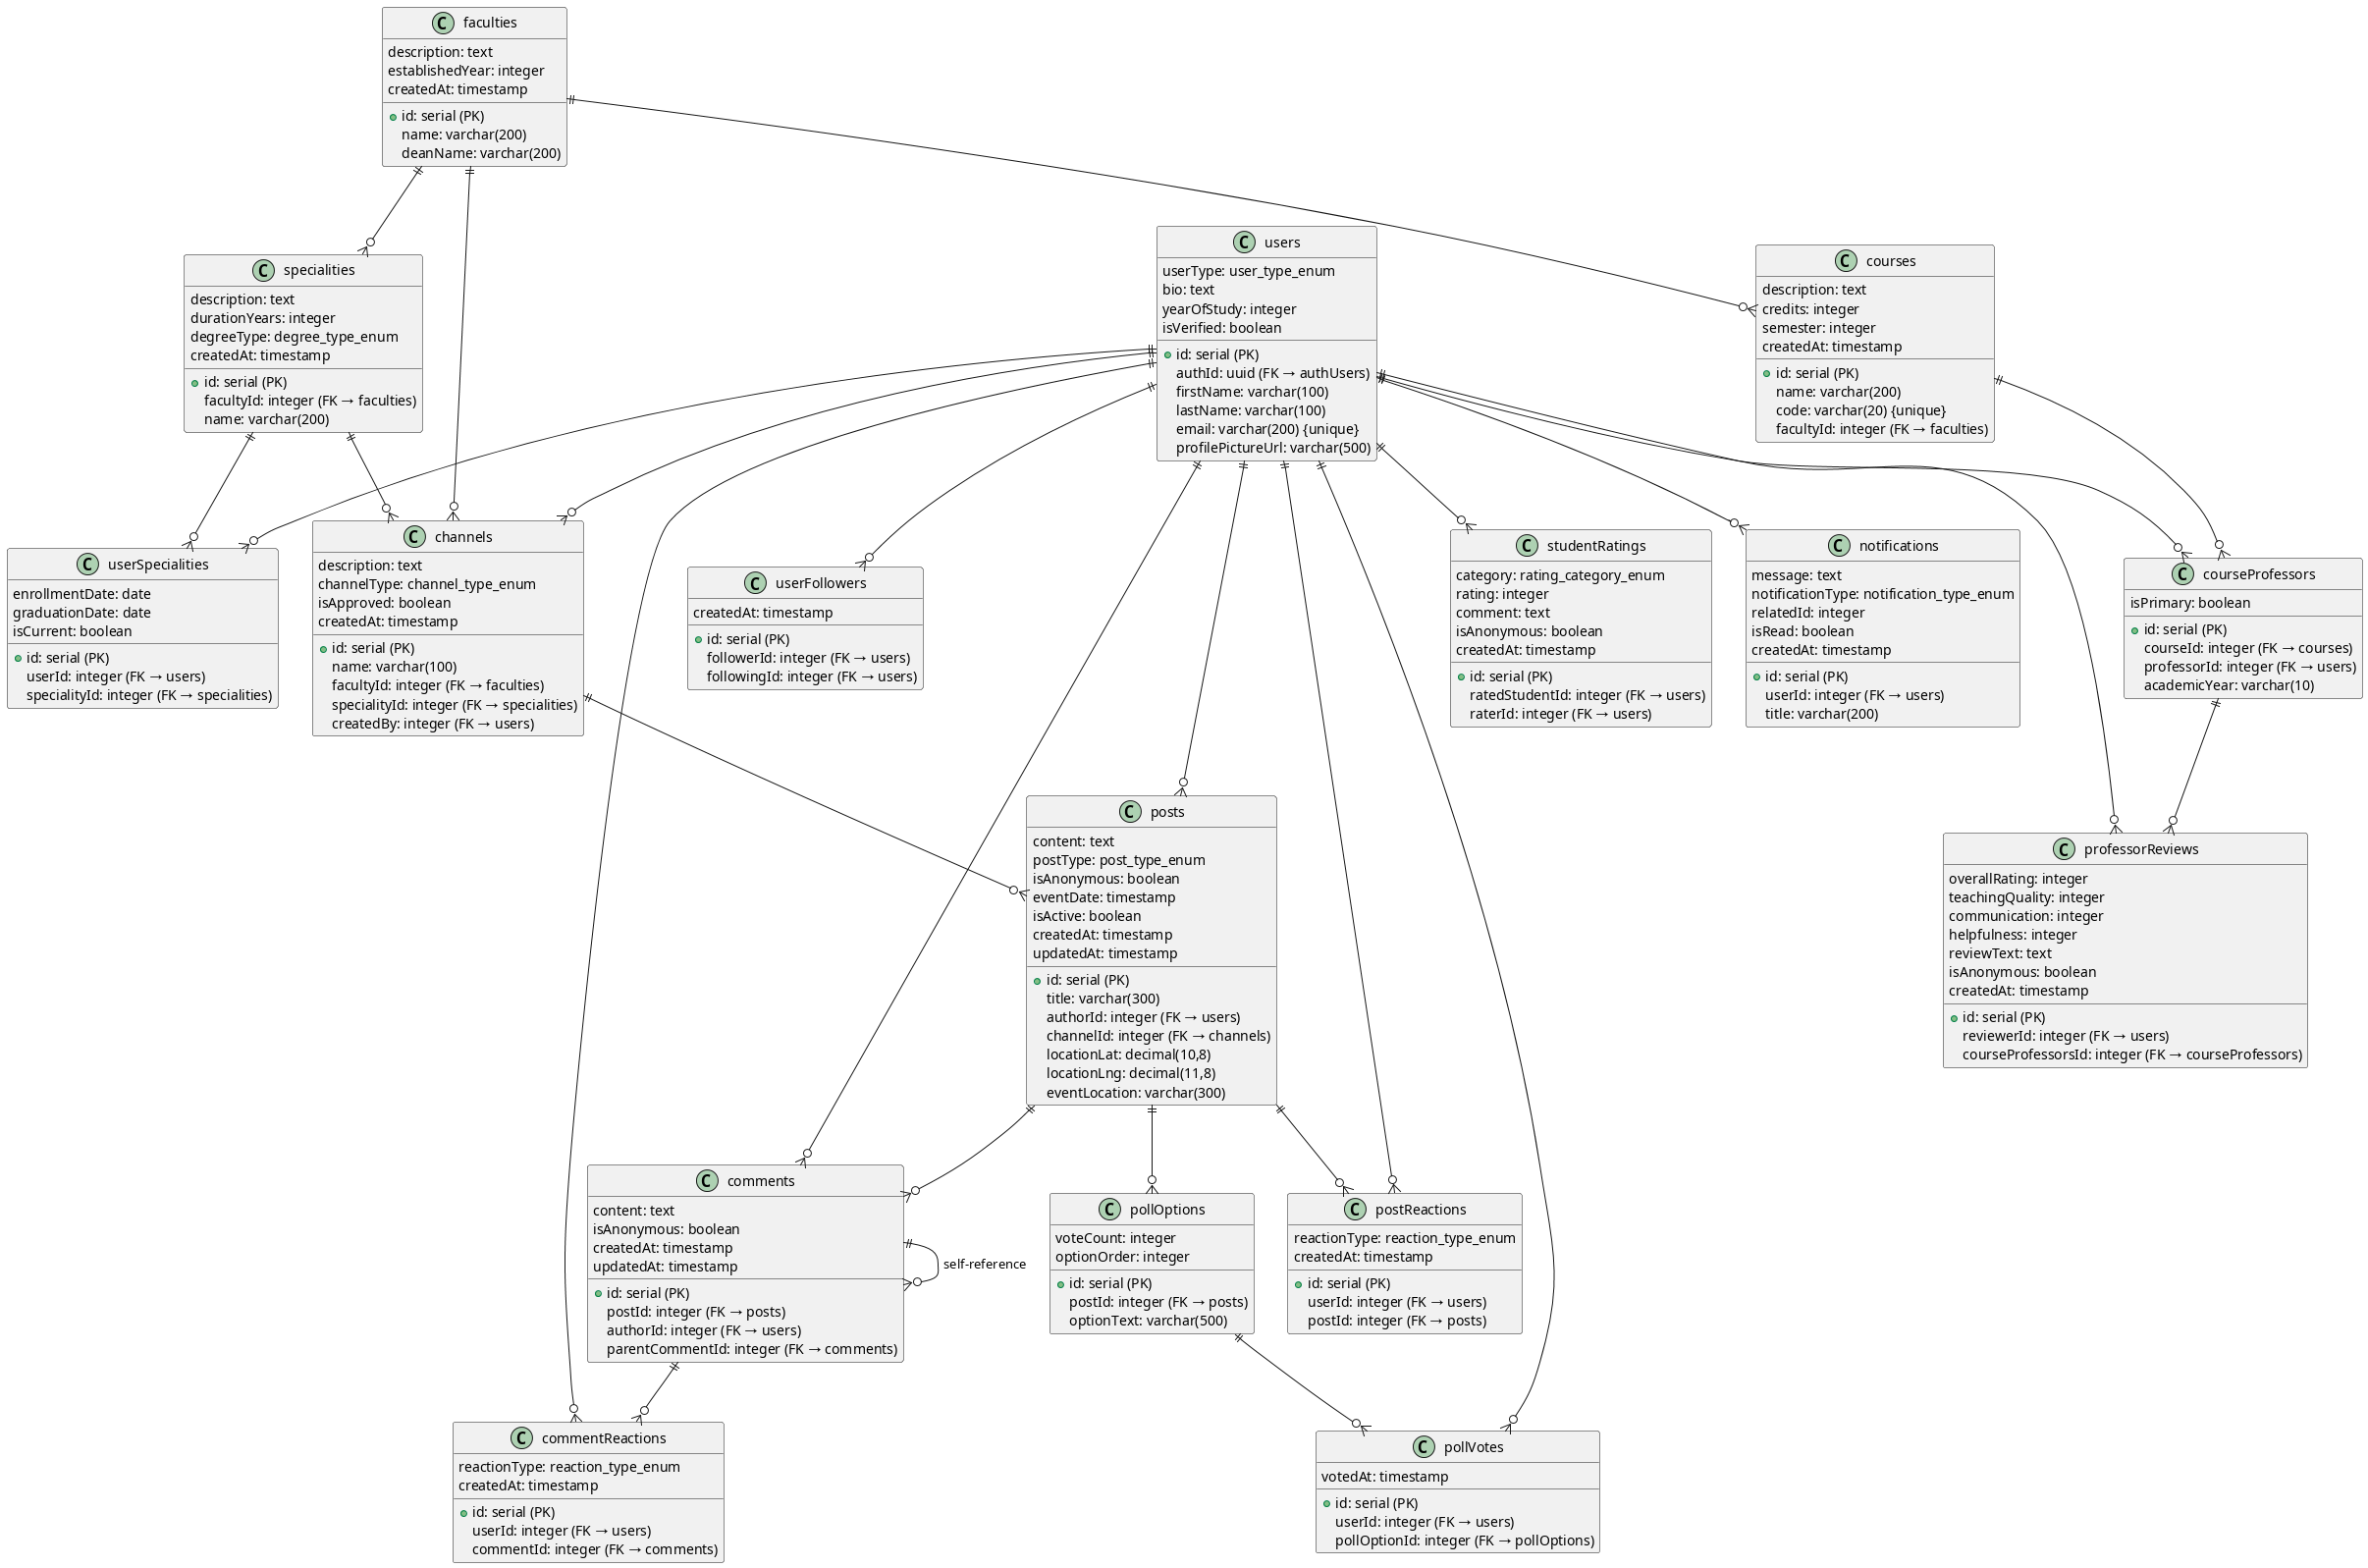
\includegraphics[width=1.0\textwidth]{img/database-schema.png}
\caption{Database Schema Class Diagram}
\label{fig:database-schema}
\end{figure}

Figure \ref{fig:database-schema} illustrates the complete database structure with entities representing users, academic faculties and specialities, forum channels and posts, and various interaction mechanisms. The schema design emphasizes referential integrity through foreign key constraints and implements proper indexing strategies for optimal query performance.

The core entities include:

\begin{itemize}
    \item \textbf{User Management}: Users table with authentication integration, supporting multiple user types (student, professor, admin) with profile information and verification status.
    \item \textbf{Academic Structure}: Faculties, specialities, and courses tables that model the university's organizational hierarchy with proper relationships and constraints.
    \item \textbf{Content System}: Posts, comments, and channels that facilitate forum discussions with support for anonymous posting, location-based content, and threaded conversations.
    \item \textbf{Interaction Features}: Reactions, ratings, polls, and social following mechanisms that enhance user engagement and content quality assessment.
\end{itemize}

\section{Security Workflows}

\subsection{User Login Process}

The login workflow implements a server-side action pattern that ensures secure authentication handling. When users submit their credentials, the system processes authentication through Supabase's secure authentication service while managing session cookies at the application level. The middleware layer automatically validates user sessions on subsequent requests, providing seamless protection for authenticated routes.

\begin{figure}[H]
\centering
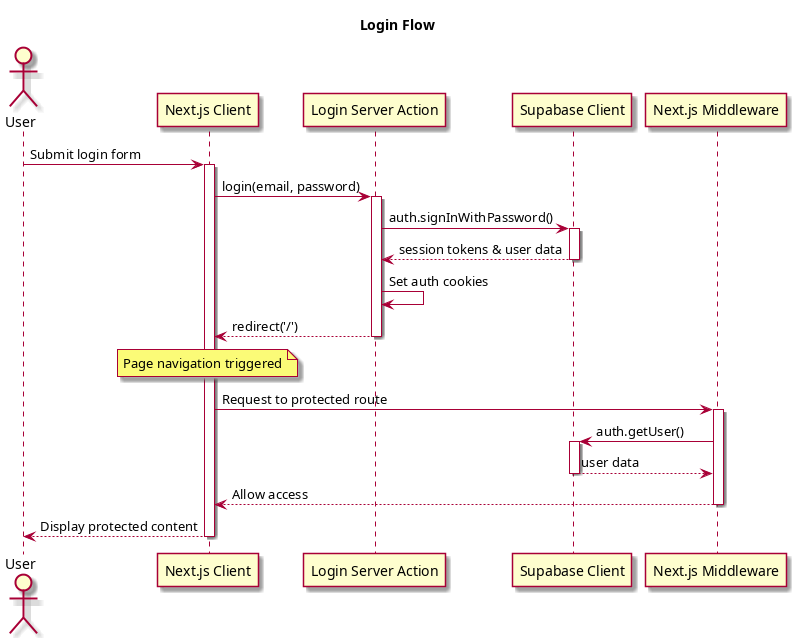
\includegraphics[width=0.9\textwidth]{img/login-sequence.png}
\caption{User Login Sequence Flow}
\label{fig:login-sequence}
\end{figure}

Figure \ref{fig:login-sequence} illustrates the complete login flow, from user credential submission through server-side validation and middleware-based route protection. The process ensures that authentication tokens are securely managed and automatically validated for protected resource access.

\subsection{User Registration Process}

The registration workflow incorporates both user profile creation and email verification processes. The system validates form data, checks for existing users in the database, and creates both authentication records and user profile information atomically. Email confirmation is handled through Supabase's built-in email service, ensuring users verify their accounts before accessing protected features.

\begin{figure}[H]
\centering
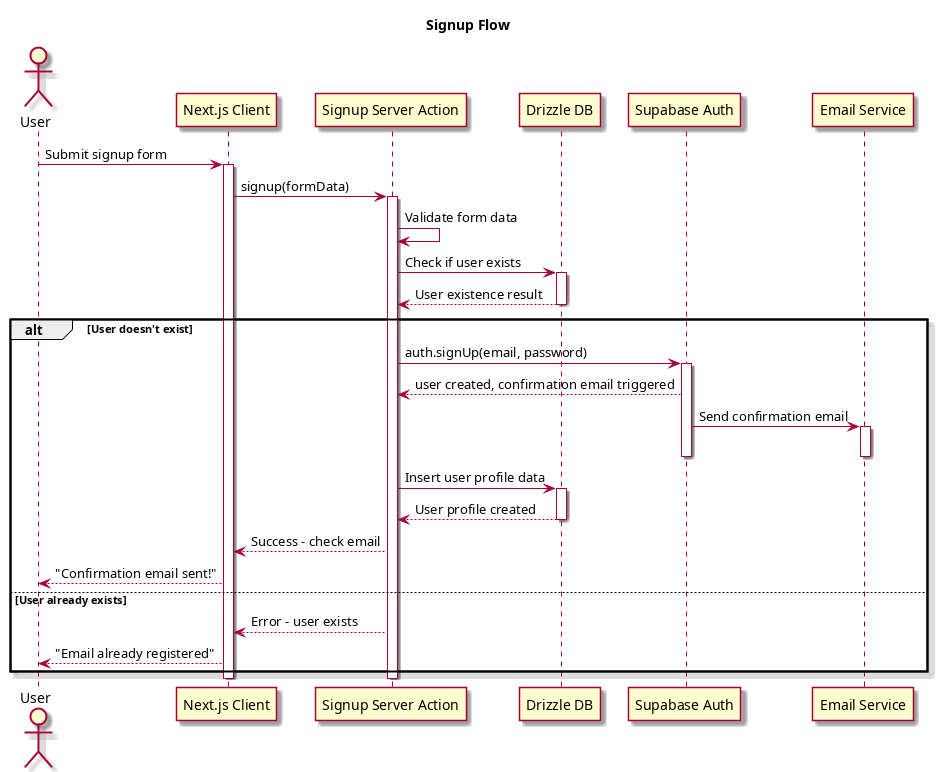
\includegraphics[width=0.9\textwidth]{img/signup-sequence.png}
\caption{User Registration Sequence Flow}
\label{fig:signup-sequence}
\end{figure}

The registration process shown in Figure \ref{fig:signup-sequence} demonstrates the integration between form validation, database operations, and email confirmation services. The system maintains data consistency by performing all operations within a controlled transaction flow.

\subsection{Email Confirmation Workflow}

Email confirmation completes the user verification process through a secure callback mechanism. When users click the confirmation link, the application processes the verification code and establishes a verified user session. This workflow ensures that only users with verified email addresses can access the platform's full functionality.

\begin{figure}[H]
\centering
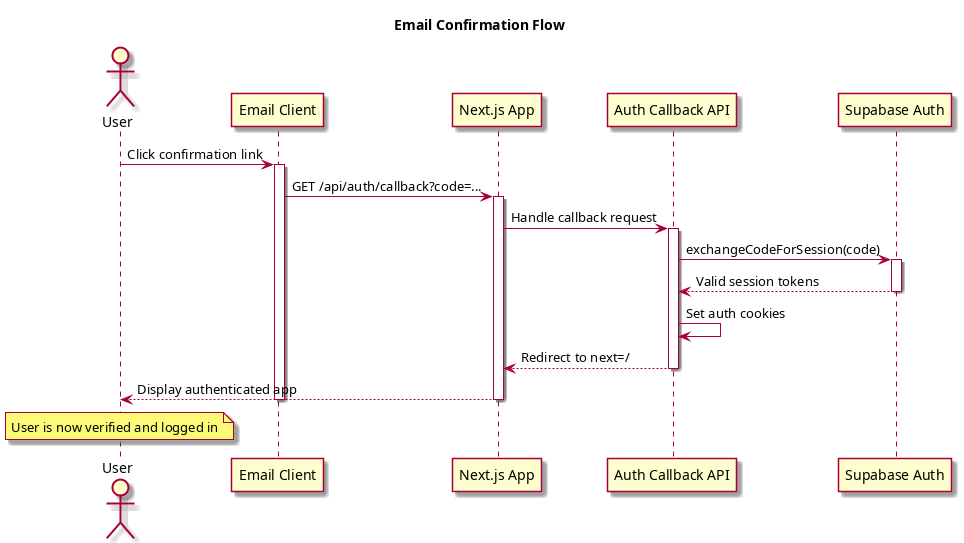
\includegraphics[width=0.9\textwidth]{img/email-confirmation-sequence.png}
\caption{Email Confirmation Sequence Flow}
\label{fig:email-confirmation}
\end{figure}

Figure \ref{fig:email-confirmation} shows the secure token exchange process that validates user email addresses and establishes authenticated sessions. The callback API handles the verification seamlessly while maintaining security best practices.

\subsection{Protected Route Access}

The middleware-based protection system automatically validates user authentication status for all protected routes. This approach provides transparent security enforcement without requiring manual authentication checks in individual route handlers. The middleware evaluates user sessions and redirects unauthenticated users to the login page while allowing authenticated users to proceed normally.

\begin{figure}[H]
\centering
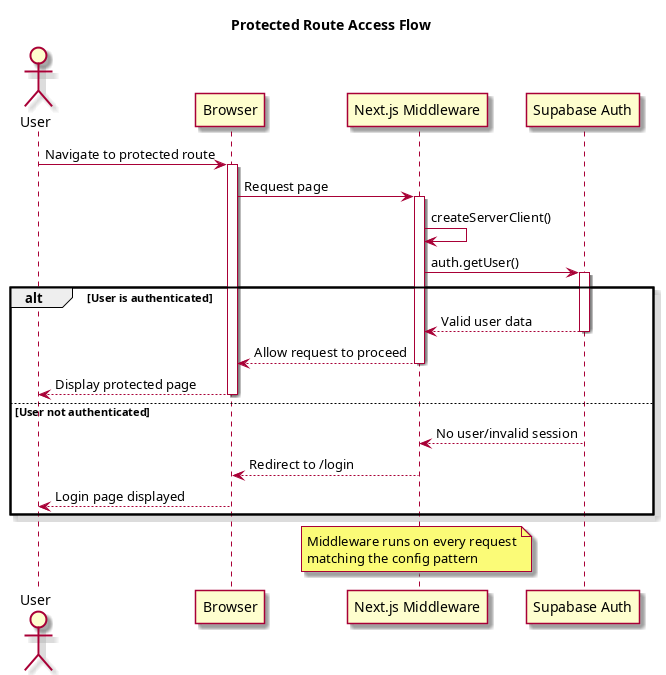
\includegraphics[width=0.9\textwidth]{img/protected-route-sequence.png}
\caption{Protected Route Access Sequence Flow}
\label{fig:protected-route}
\end{figure}

The protection mechanism illustrated in Figure \ref{fig:protected-route} ensures consistent security enforcement across the application. The middleware pattern provides a centralized authentication checkpoint that automatically handles both authenticated and unauthenticated access scenarios.